\documentclass[master=mai,masteroption=ecs]{kulemt}
  \setup{title={Complete decision tree induction functionality in scikit-learn},
  author={Ir.\ Sven Van Hove},
  promotor={Prof.\,dr.\ Jesse Davis \and Prof.\,dr.\,ir.\ Hendrik Blockeel},
  assessor={Dr.\,ir.\ Marc Claesen},
  assistant={Elia Van Wolputte}}
  
  \setup{filingcard,
  translatedtitle=Complete beslissingsboom inductie functionaliteit in scikit-learn,
  udc=681.3*I20,
  shortabstract={500 word abstract}} %TODO copy abstract
  
  % \setup{coverpageonly}
  
  \setup{font=lm}
  
  \usepackage[pdfusetitle,colorlinks,plainpages=false]{hyperref}
  \usepackage{nameref}
  \usepackage{amsmath}
  \usepackage{amssymb}

\begin{document}

\begin{preface}
  I would like to thank Elia for the insightful discussions after business hours. I would also like to thank prof.\ Davis and prof.\ Blockeel for their helpful suggestions and the full jury for taking to time to read this document. My sincere gratitude also goes to my family and friends for their continued support. Finally, I would like to show appreciation towards my employer for the flexibility in my work schedule that made obtaining this degree possible.
\end{preface}

\tableofcontents*

\setlength{\parindent}{0cm}
\setlength{\parskip}{2ex plus 1ex minus 1ex}

% # APPROACH:
% 1. Investigate and characterize the differences in functionality between Weka and scikit-learn for decision trees.
% 2. Implement a python version of a decision tree learner that has the required basic functionality and that uses the scikit-learn interfaces.
% 3. Benchmark the developed implementation to those available in scikit-learn and Weka on a suite of datasets.
% 4. Translate the python implementation to C/cython in order to improve the run time performance.
% 5. Extend the decision tree implementation to more advance settings (e.g., online learning, …).
% 6. Provide good documentation on how the code works.

\begin{abstract} %TODO update abstract
  The \texttt{abstract} environment contains a more extensive overview of
  the work. But it should be limited to one page.~\cite{eibe2016weka}
\end{abstract}

\mainmatter%

\chapter{Introduction}\label{cha:intro}

\section{Context}
Decision tree induction is one of the most well-known tools in the machine learning community. Most of the theoretical groundwork was laid in the last three decades of the previous century. Researchers Leo Breiman and Ross Quinlan have been particularly influential in this space. Some well-know algorithms include the Concept Learning System (CLS)~\cite{cls} and ID3~\cite{id3, id3bis, id3ter} by Quinlan, and Classification And Regression Trees (CART)~\cite{cart} by Breiman. 

Contemporary AI researchers focus a lot of their attention on neural networks and in particular deep learning --- the recent hype around DeepMind's AlphaGo~\cite{alphago} victories comes to mind. Nevertheless, a quick Google Scholar search will reveal that decision tree research is not dead. Researchers still continue to propose new or improved algorithms and analyses.

Theory is one thing, but the algorithms need to be implemented as computer programs to actually be useful. Scikit-learn~\cite{scikit-learn} is a very popular machine learning library written in Python. As such, it also contains implementations of various decision tree induction algorithms. Before scikit-learn became popular, a Java-based library called Weka~\cite{eibe2016weka} (or ``Waikato Environment for Knowledge Analysis'' in full) was often used instead. The implementations of decision tree algorithms in Weka are to this day still in many respects superior to those in scikit-learn. Other libraries that implement similar algorithms exist (e.g., Apache Spark~\cite{spark}), but those are beyond the scope of this text.

\section{Goal}
The goal of this thesis is to alleviate the discrepancies between scikit-learn and Weka concerning decision tree induction. Mind that decision tree induction tools can never be truly ``complete'' as stated in the title because the field is immensely broad and still continues to grow. Nevertheless, an effort can be made to improve feature parity between these two popular tools.

One such discrepancy was found when comparing the performance of decision tree induction algorithms in Weka and scikit-learn on an activity dataset~\cite{problematic_dataset}. The difference between classification accuracies in this case was considerable at about 25\% in favour of Weka.

\section{Motivation}
Some would perhaps question the relevance of such ``outdated'' techniques anno 2018. This feeling is misguided. The advantages of decision tree induction algorithms are still hard to compete with, even for more modern algorithms~\cite{scikit-learn, murthy1998automatic, kotsiantis2007supervised}:

\begin{enumerate}
    \item Comprehensible: makes intuitive sense even for the uninitiated.
    \item Transparent, as opposed to for example artificial neural networks
    \item Easy to visualize (if number of nodes remains small)
    \item Non-parametric: makes very few assumptions about data
    \item No data normalization required
    \item Handles both categorical and numerical data
    \item Handles missing data elegantly %TODO missing values fix?
    \item Handles multiclass, multilabel and multioutput problems natively
    \item Fast training
    \item Fast inference
\end{enumerate}

Of course decision tree induction algorithms are not perfect:
\begin{enumerate}
    \item Unstable: small modifications in training data can result in a completely different tree
    \item Learning optimal trees is an NP-Complete problem~\cite{npcomplete}, so heuristics are used to find approximations
    \item Prone to overfitting if not actively countered by adding early stopping criteria or an extra pruning step
    \item Prone to bias when one class appears more much frequently in the training set than others.
\end{enumerate}

Some of these drawbacks can be overcome by using an ensemble of decision trees, but that in turn negatively impacts some of the advantages.

\section{Thesis structure}
The structure of the remainder of this text is as follows. First, an overview of the literature study concerning decision tree induction will be presented and the scope of the thesis will be determined. Next, the decision tree implementations in Weka and scikit-learn are compared to their underlying algorithms and to each other. This results in a list of capabilities. Based on these differences in capabilities, we formulate some hypotheses that can explain the differences in performance. Chapter~\ref{cha:method} discusses experimental setups. It is followed by chapter~\ref{cha:results} which presents and discusses the results of these experiments. We conclude with chapter~\ref{cha:conclusion}.
%TODO improve structure
\chapter{Literature review}\label{cha:literature}
The relevant literature for this thesis mostly consists of papers concerning decision tree induction. These go back many decades, but fortunately there are some review and survey papers that provide a convenient overview~\cite{murthy1998automatic, rokach2005top, kotsiantis2007supervised}. On top of the academic literature, the source code and accompanying documentation of scikit-learn and Weka have also been a rich source of information.

\section{Prerequisites}
The reader ought to be familiar with basic machine learning concepts such as supervised learning, classification, regression, overfitting, model validation and ensemble learning. Furthermore, elementary knowledge of decision tree induction is expected. The most important basic concepts will briefly be recapitulated. Topics that are particularly important for the next chapters will be elaborated on.

\section{Scope}
A wide variety of decision tree induction algorithms exists. Here, only the \emph{top down induction of decision trees (TDIDT)} family is considered. It is the most common approach and it is particularly relevant to the software tools under scrutiny.

Unsupervised and semi-supervised algorithms are out of scope. Furthermore, only classification trees are considered. With little effort, most TDIDT classification algorithms can be converted to regression algorithms. Yet, these are far less popular than their classification counterparts and better alternatives such as XGBoost~\cite{xgboost} exist.

Ensemble methods are also out of scope. Recent decision tree algorithms rarely work with a single (complex) tree, but rather with an ensemble of relatively simple trees. Random forests~\cite{rf} is a very popular example of bootstrap aggregating or \emph{bagging}. Regardless, the scope of this thesis concerns the fundamentals of decision trees, and not their derivatives. On the other hand, implementation improvements suggested in this thesis can potentially benefit related ensemble methods. Other derivatives that are out of scope include logic trees and model trees.

The algorithms in scope are all offline learning methods. This is also known as batch learning. It implies that all computation is done in one place and that all data has to fit in memory. Online learning has gained relevance in the big data era since it does not impose such restrictions. On the other hand, the technique is only used if the context requires it because the performance is not up to par with offline learning.

Finally, only univariate tests are in scope. The test performed in each internal node must only evaluate one attribute of the observation. For categorical attributes, this typically implies checking whether or not the input is equal to a fixed category. For numerical (and thus ordered) attributes, the input value is compared against a fixed threshold using the less than or equal operator. Consequently, the input space is partitioned recursively using axis-aligned hyperplanes. This scope limitation precludes well-known but unpopular extensions such as oblique trees.

\section{Terminology}
Throughout the relevant literature, there is a lack of ubiquitous vocabulary shared by all researchers. Decision trees are used in various scientific fields, each of which has its own jargon. Specifically, there is a big divide between researchers that approach the problem from a machine learning perspective compared to those who come from a statistics background. To avoid confusion, we avoid synonyms and always use the same term for the same concept. In the following paragraphs, some basic terms are reviewed. 

A \emph{decision tree} consists of \emph{(internal) nodes} which are connected to other nodes via a one-to-many \emph{parent-child} relation on one hand, and \emph{leaves} which have no children on the other hand. The \emph{root node} is the only node without parent. In a \emph{binary tree}, all internal nodes have two children.

Induction algorithms typically receive a \emph{training set} as input data to construct a decision tree while a \emph{test set} is used afterwards for model validation. These sets are tables of data where each row represents an \emph{observation}. All observation are fully described by a common set of \emph{attributes}. Some attributes are \emph{categorical}, others may be \emph{numerical}.\footnote{The latter is sometimes also referred to as \emph{ordered} because this is the underlying property of numbers the algorithm will exploit at some point. Strictly speaking categories can also have an implicit order. In that case, a good practice is to make this explicit by numerically encoding them beforehand.} In a supervised learning context, one or more \emph{target attributes} are present. For classification tasks, target attributes are considered categorical even if they contain numeric data. The distinct values of a target attribute are called the \emph{class labels} of that attribute. A classification task is called \emph{binary classification} if there is exactly one target attribute which has exactly two associated class labels and each observation is associated with exactly one of the two class labels. If multiple class labels can be associated with an observation, the task is called \emph{multilabel classification}. If instead there are more than two class labels, it is referred to as \emph{multiclass classification}. \emph{Multioutput classification} on the other hand occurs when multiple target attributes, each with their own distinct set of class labels, have to be derived from the same set of (non-target) attributes. This can be accomplished trivially by creating multiple trees, each handling one class. However, combining them in one tree might offer performance benefits~\cite{vens2008decision, multioutput-better}. Decision trees are one of the few machine learning algorithms that can handle all these modes of operation natively.

During \emph{fitting}, first one root node is created and all observations in the training set are stored in this node. When a node is \emph{split} using some \emph{test function}, this function partitions the observations in subsets and then creates a child node for each subset. This process is repeated recursively until some stopping criterion is reached. The \emph{purity} of a node is defined as the percentage of observations in that node that belong to the majority class. A \emph{pure node} is a node with 100\% purity. When the tree is complete, it can \emph{predict} the output based on input from, for example, the test set.

\section{A generic TDIDT algorithm}
A typical TDIDT algorithm for classification consists of two phases: a grow phase and an optional prune phase. The grow phase requires three subroutines with fixed signatures: a test generation subroutine, a node splitting subroutine and a stopping subroutine. Historically, researchers presented their TDIDT algorithms with fixed subroutines. Because of the shared interface it is now common to choose these subroutines \emph{\`{a} la carte}. One could try to evaluate the performance of each subroutine separately, but selecting the best subroutine for each slot separately does not guarantee a global optimum. Holistic tests must be performed to ensure the best configuration is chosen. Also note that the efficacy of each combination seems to depend on the domain in which it is applied~\cite{mingers1989empirical}.

\subsection{Univariate test generation}
Based on the set of observations in a node, tests can be devised that partition this set in a number of subsets. The goal of this step is to generate a finite number of tests $\tau_i \in \mathcal{T}$ based on one associated attribute. Recall the tests based on multiple attributes exist but are out of scope. In the next step, one specific test is chosen from this set of possible tests.

Generating tests for categorical attributes is trivial. For binary trees, each test compares its input (i.e., the value of the associated attribute of an observation) against one fixed value selected from all known values of the associated attribute. If the test is positive, the observation belongs to the first subset, else to the second. This results in as many tests as there are possible values for the associated attribute. For non-binary trees, one test suffices that maps each distinct attribute value to a specific subset. Figures~\ref{fig:categorical_binsplit} and~\ref{fig:categorical_split} illustrate the difference. Non-binary trees are typically shallower and thus faster to go through from top to bottom during the inference phase. On the other hand, it is an all-or-nothing approach. If an attributes contains 100 different categories where only a few of them are very relevant, is it worth it to add 100 child nodes to the current node? Binary trees have more flexibility in this regard, but they pay for it in depth.

\begin{figure}[htp]
\begin{center}
    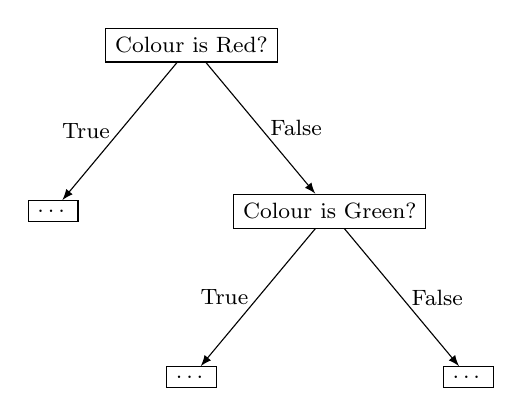
\begin{tikzpicture}
        [
            boxed/.style         = {shape=rectangle, draw, align=center},
            sibling distance        = 10em,
            level distance          = 6em,
            edge from parent/.style = {draw, -latex},
            every node/.style       = {font=\footnotesize},
            ]
            \node [boxed] {Colour is Red?}
            child { node [boxed] {\ldots} edge from parent node [left] {True} }
            child { node [boxed] {Colour is Green?}
            child { node [boxed] {\ldots} edge from parent node [left] {True} }
            child { node [boxed] {\ldots} edge from parent node [right] {False} }
            edge from parent node [right] {False} 
            };
        \end{tikzpicture}
    \end{center}
    \caption{Example of nodes that perform binary tests associated with the attribute Colour. Two levels are needed to reach the same conclusion as in \autoref{fig:categorical_split}. Of course in practice not every value is equally relevant, so it is difficult to make statements about which approach is better without knowing the context.}%
    \label{fig:categorical_binsplit}
\end{figure}
    
\begin{figure}[htp]
\begin{center}
    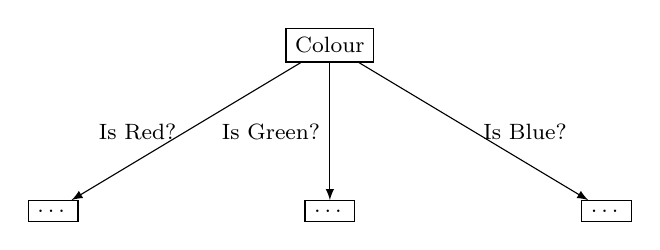
\begin{tikzpicture}
        [
            boxed/.style         = {shape=rectangle, draw, align=center},
            sibling distance        = 10em,
            level distance          = 6em,
            edge from parent/.style = {draw, -latex},
            every node/.style       = {font=\footnotesize},
            % every node/.style = {shape=rectangle, draw, align=center}
            % sloped
        ]
        \node [boxed] {Colour}
            child { node [boxed] {\ldots} edge from parent node [left] {Is Red?} }
            child { node [boxed] {\ldots} edge from parent node [left] {Is Green?} }
            child { node [boxed] {\ldots} edge from parent node [right] {Is Blue?} };
    \end{tikzpicture}
\end{center}
\caption{Example of a node that performs a test associated with the attribute Colour. Since this target attributes contains three distinct class labels, the observations are partitioned over three child nodes.}%
\label{fig:categorical_split}
\end{figure}

In the case of numerical attributes, thresholds are introduced to partition the observations based on the implied ordering. That way, an infinite number of tests can be generated, which is of course undesirable. However, at least for the training set, not all tests will result in a different partitioning. A clever choice of thresholds should bring the number of subsets back to a manageable level. \autoref{fig:numerical_split} shows an example.

\begin{figure}[htp]%
\label{fig:numerical_split}
\begin{center}
    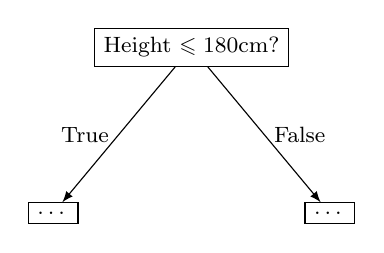
\begin{tikzpicture}
        [
            boxed/.style         = {shape=rectangle, draw, align=center},
            sibling distance        = 10em,
            level distance          = 6em,
            edge from parent/.style = {draw, -latex},
            every node/.style       = {font=\footnotesize},
        ]
        \node [boxed] {Height $\leqslant 180$cm?}
            child { node [boxed] {\ldots} edge from parent node [left] {True} }
            child { node [boxed] {\ldots} edge from parent node [right] {False} };
    \end{tikzpicture}
\end{center}
\caption{Example of a node that performs a test associated with the numerical attribute Height. In this case a threshold of 180cm was chosen, but of course any threshold is allowed as long as it divides the set of all height values in two non-empty subsets.}
\end{figure}

%attribute selection > splitting

\subsection{Splitting}
Classic TDIDT algorithms work by recursively splitting nodes based on some optimal test $\tau \in \mathcal{T}$, the set of all possible tests. A heuristic called the splitting criterion is required to determine this $\tau$. A few such criteria have stood the test of time.

\subsubsection{Purity}
Given the set of all associated observations of a node $S$, the perfect test $\tau^*$ induces a partition $\mathcal{S}_{\tau^*} = \{S_1, \ldots, S_k\}$ wherein each subset is pure, so optimizing for weighted average partition purity is a sensible first criterion.

\begin{equation}
    p(\mathcal{S}_\tau) = \sum_i \frac{|S_i|}{|S|} p(S_i)
\end{equation}

Here, $S = S_1 \cup \ldots \cup S_k$ and $p(S)$ is the set purity as described above.
%can also be expressed as impurity instead using the same pattern as below

\subsubsection{Entropy and information gain}
In practice purity does not appear to work very well. That is why researchers came up with an alternative based on Shannon's information theory~\cite{shannon1948mathematical}. Quinlan used such metrics in many of his prominent algorithms such as ID3 and C4.5~\cite{id3ter, c45}, but it was already invented earlier for the Concept Learning System (CLS)~\cite{cls}. Define entropy (or missing information) of a variable $V$ with possible values $v_i$ and associated probabilities $p(v_i)$ as follows:

\begin{equation}
    s(V) = - \sum_i p(v_i) \log_2(p(v_i))
\end{equation}

The same principle can also be applied to a set. When we do this for the set of observations $S$ and the classes $c_i$ associated with those observations, the class entropy $s_C(S)$ is defined as follows:

\begin{equation}
    s_C(S) = - \sum_c p(c) \log_2(p(c))
\end{equation}

where $p(c)$ is the probability that a random observation in $S$ belongs to class c. This value can be defined for any node, independent of any specific partition.

For a given test $\tau$, a similar definition can be given for each subset $S_i$ of the induced partition on $S$:

\begin{equation}
    s_C(S_i) = - \sum_c p_i(c) \log_2(p_i(c))
\end{equation}

For the entropy of the whole partition $\mathcal{S}_\tau$, again use the weighted average entropy of its subsets:

\begin{equation}
    s_C(\mathcal{S}_\tau) = \sum_i \frac{|S_i|}{|S|} s_C(S_i)
\end{equation}

Finally, calculate the information gain $h_{IG}(\tau, S)$ of the split that resulted from test $\tau$:

\begin{equation}
    h_{IG}(\tau, S) = s_C(S) - s_C(\mathcal{S}_\tau)
\end{equation}

where $\mathcal{S}_\tau$ is the partition resulting from test $\tau$.

\subsubsection{Gain ratio}
The information gain criterion is biased towards tests with many possible outcomes~\cite{harris2002information}. This could be a problem in non-binary trees. The gain ratio alleviates this problem. First define split information $SI(\tau, S)$ --- the maximum possible information gain --- as follows:

\begin{equation}
    SI(\tau, S) = - \sum_i \frac{|S_i|}{|S|} \log_2 \frac{|S_i|}{|S|}
\end{equation}

Finally, define the gain ratio:

\begin{equation}
    h_{GR}(\tau, S) = \frac{h_{IG}(\tau, S)}{SI(\tau, S)}
\end{equation}
%watch out for instability due to very low SI! -> only calculate when high enough

In binary trees, this heuristic typically causes a less balanced tree compared to the information gain criterion~\cite{c45}.

\subsubsection{Gini}
Distance metrics such as the Gini impurity index can be used instead of heuristics based on information theory~\cite{cart}. The definitions follow the same pattern as those of the information gain:

\begin{equation}
    g(S) = \sum_c p(c)(1 - p(c))
\end{equation}
\begin{equation}
    g(S_i) = \sum_c p_i(c)(1-p_i(c))
\end{equation}
\begin{equation}
    g(\mathcal{S}_\tau) = \sum_i \frac{|S_i|}{|S|} g(S_i)
\end{equation}
\begin{equation}
    h_G(\tau, S) = g(S) - g(\mathcal{S}_\tau)
\end{equation}

% \subsubsection{Comparison}

\subsection{Early stopping}
Breiman argues in his CART book~\cite{cart} that choosing good early stopping criteria is far more important than choosing good splitting criteria. If early stopping was not applied or no pruning (see below) was performed afterwards, trees would grow excessively large on real world data sets. This is a classic case of overfitting. It negatively impacts many factors that make decision trees attractive in the first place, such as their comprehensibility and their quick fitting and predicting. It is also detrimental to the performance of the model on unseen data since the model fails to generalize properly.

There are simple and more complex stopping criteria. Simples ones are based on statistics such as these:
\begin{enumerate}
    \item tree depth
    \item number of leaves
    \item number of observations in a node
    \item purity of a node
\end{enumerate}

More complex stopping criteria can be based on the Minimum Description Length (MDL) of a tree~\cite{mdlstopping} or on statistical techniques such as a $\chi^2$-test. Quinlan proposed to use the latter in his ID3 algorithm but decided not to include it in the successor C4.5~\cite{id3ter, c45} due to its unreliability.

\subsection{Pruning}
A better alternative to early stopping criteria is to let the tree grow freely, and to prune it afterwards in a bottom-up fashion. Typically, the current error estimate of the subtree rooted at the given node is compared to what the estimated error would be if this node was converted to a leaf by pruning away its descendants. If it would perform better as a leaf, the descendants are effectively pruned away. Many different pruning algorithms exists. What follows is a non-exhaustive list of common pruning approaches.

\subsubsection{Reduced Error Pruning}
Reduced Error Pruning (REP) is one of the most straightforward and statistically sound methods of pruning a tree~\cite{quinlan1987simplifying, repanalysis}. Instead of using the whole training set to grow the tree, some randomly chosen observations are withheld in a separate validation set. By using this validation set after the growth phase is completed, an unbiased estimate of the error of each node in the tree can be calculated. Nodes at the bottom of the tree are converted into leaves if the estimated error of the leaf is equal to or less than the estimated error of the subtree rooted at the given node. This process is repeated recursively until the smallest possible tree is obtained with the minimum estimated error based on the validation set.

The disadvantage of this method is that less data is available for growing the tree, potentially negatively impacting this process. This is not a concern if training data is available in abundance.

\subsubsection{Error Based Pruning}
Error Based Pruning (EBP) is a technique used in C4.5~\cite{c45}. It does not require a separate validation set, so the full training set can be used to grow the tree. The downside of this is that this method is less statistically sound because it is impossible to calculate an unbiased estimate of the error. Instead, an upper bound is calculated based on the training error and that upper bound is used instead of the original error in comparisons. Generally speaking, if a node is associated with fewer observations then there is less certainty about the error and the upper bound will be further away from the original value. The calculation also depends for a large part on the required level of confidence, which the user must provide.

\subsubsection{Cost Complexity Pruning}
Cost Complexity Pruning, used in the CART algorithm~\cite{cart}, takes another approach akin to regularization in classic optimization problems. First, it generates a series of pruned trees based on the original. Then it considers both the total training error and a cost factor proportional to the size of each tree to make a first selection. If the training error increases due to the pruning, but it is compensated for by a much smaller tree, the operation as a whole can still be considered positive depending on a trade-off factor. The final tree is chosen from this first selection using a separate validation set. As such, the same drawbacks apply here as for Reduced Error Pruning.

\subsubsection{Others}
Many other pruning algorithms exist~\cite{mingers1989empirical, breslow1997simplifying, elomaa1999biases, esposito1997comparative}. The reader can find some inspiration in the following list:

\begin{enumerate}
    \item Minimum error pruning~\cite{niblett1986learning}
    \item Pessimistic pruning~\cite{mansour1997pessimistic, quinlan1987simplifying, c45}
    \item MDL-based pruning~\cite{mdlpruning, quinlan1989inferring}
    \item Critical Value Pruning~\cite{mingers1987rule}
    \item Pruning using back propagation~\cite{backproppruning}
\end{enumerate}

\subsubsection{Alternative: Rule-based Pruning}
An outlier in this list is Rule-based Pruning. Decision trees can be converted to a series of if-then statements where the condition is a conjunctive clause. These statements can be further simplified to if-then-else statements and then optimized, which can be seen as an alternative form of pruning. The resulting model is no long a tree, so it is considered out of scope for this thesis, but it can still approximate the underlying concept that the tree used to represent.

\section{Conclusion}
TDIDT algorithms incorporate different subroutines, for each of which a number of alternatives are available. This makes them a very flexible tool with uses in a variety of settings. Popular algorithms such as C4.5 and CART are opinionated in the sense that they each propose a small number of specific configurations of components. Fortunately, that does not stop algorithm implementers from offering more choice to their users, as shown in the next chapter. Note also that there is no single precise definition of ID3, C4.5 or CART. New insights were acquired over time and added to the solution, but the algorithm name rarely changed.
\chapter{Existing implementations}\label{cha:software}
Chapter~\ref{cha:literature} briefly discussed the theoretical basics of decision trees. In this chapter, we consider applications of this theory in the form of two popular software libraries: Weka~\cite{eibe2016weka} and scikit-learn~\cite{scikit-learn}.

\section{Capabilities}
The most important difference between the two libraries regarding decision trees is in the base algorithm they started from. The J48 algorithm in Weka is based on Quinlan's C4.5~\cite{c45}, while the \texttt{DecisionTreeClassifier} in scikit-learn used CART by Breiman~\cite{cart} as the foundation. This has a profound impact on the capabilities of both implementations. These capabilities are divided in categories and discussed one by one in the following subsections.

\subsection{Structural capabilities}
CART only supports binary trees, and the same applies for scikit-learn's implementation. It is an option in J48, but the default settings generate non-binary trees. Binary trees are typically deeper than their non-binary counterparts, making the inference phase more computationally expensive. On the other hand, Elomaa et al.\ claim that the use of binary discretization with C4.5 needs about the half training time of using C4.5 multisplitting~\cite{elomaa1999general}. Note that this only impacts splits on categorical attributes; splits of numerical attributes are always binary.

\subsection{Input capabilities}
\subsubsection{Categorical and numerical attributes}
\label{sssec:cat_num_attr}
ID3 was not capable of dealing with numerical attributes, but C4.5 and CART can handle both types. J48 can also handle both just like its theoretical counterpart C4.5. Scikit-learn's implementation however did not inherit the categorical input capabilities of CART. This is understandable from a software engineering perspective: scikit-learn is built on top of numpy~\cite{numpy} which itself is a numeric, scientific computing library. The user can work around this issue by pre-processing the categorical data, using for example a \texttt{LabelEncoder}\footnote{\url{http://scikit-learn.org/stable/modules/generated/sklearn.preprocessing.LabelEncoder.html}} to map each category onto a unique ID or a \texttt{OneHotEncoder}\footnote{\url{http://scikit-learn.org/stable/modules/generated/sklearn.preprocessing.OneHotEncoder.html}} that introduces as many boolean dummy variables as there are categories where only one is active at any given category.

Consider an example where an attribute Colour contains three categories: Red, Green and Blue. By default Weka would generate a single test out of this attribute. Red would be mapped to the first child, green to the second and blue to the third. This is not possible in scikit-learn because it is based on CART which only generates binary trees. CART --- which can handle categorical attributes in theory --- would generate three tests instead for attribute $x$: $(x == \text{Red})$, $(x == \text{Green})$ and $(x == \text{Blue})$. Each test has a boolean output which decides whether to jump to the left or the right child. 

In scikit-learn, the one-hot encoder would replace the Colour attribute with three numerical dummy attributes: ColourRed, ColourGreen and ColourBlue. In this case, Red is represented as [1, 0, 0], Green as [0, 1, 0] and Blue as [0, 0, 1]. Because these are numerical attributes, the test generation function will try to find thresholds to partition the space. In this case, only one threshold somewhere between 0 and 1 (e.g., 0.5) is needed. As such, each dummy variable will cause the generation of one test: $(x \leqslant 0.5)$. Although the implementation is slightly different, there is a trivial isomorphism between these three tests and the three CART tests. Consequently, the semantics are preserved even though they are slightly obscured.

Alternatively, the label encoder would replace this categorical attribute with a single numerical attribute with possible values 0, 1 and 2. This implies that there is an order among the colours, which is not supposed to be the case. Tests such as $(x \leqslant 1.5)$ could be generated. This is equivalent to $(x == \text{Red} \lor x == \text{Green})$, which is more expressive then what was possible so far. That looks positive at first, but not all logical combinations can be representation this way. Even worse, what can be represented depends entirely on the non-existent order of the original categorical variable. In short, this technique does not adhere to the original semantics and should not be used.

In conclusion, the suggested workaround with the one-hot encoder is acceptable but that does not change the fact that it negatively impact two of the decision tree advantages we listed earlier in \autoref{cha:intro}: no data preparation required and excellent comprehensibility.

\subsubsection{Missing values}
Another important input capability is dealing with missing values. As stated before, decision trees have fairly straightforward ways of dealing with this problem. While the papers on ID3 ignored this issue, both C4.5 and CART have methods for dealing with it. As before, Weka inherited the capability from C4.5, but scikit-learn did not inherit the same from CART. This is another case where extra pre-processing is needed to make decision tree induction work with scikit-learn. During this process, valuable observations might be thrown out entirely.

\subsection{Output capabilities}
Regression is not supported by C4.5 and consequently not a capability of Weka's J48. For this thesis regression is out of scope, but it is still an important point. Note however that Weka contains other decision tree algorithms, some of which do accommodate regression.

%TODO multiclass, multilabel, multioutput
%TODO model trees? ~ regression

\subsection{Splitting criteria}
Another difference lies in the choice of splitting criteria. C4.5 and J48 support the typical criteria based on information theory such as information gain and gain ratio. CART and scikit-learn on the other hand both support information gain and the Gini impurity index but not gain ratio since it is not beneficial for binary trees. The purity criterion is not implemented in any of the algorithms due to its poor performance.

\subsection{Early stopping and pruning}
As mentioned at the end of \autoref{cha:literature}, both C4.5 and CART seemingly have their favourite pruning algorithms. The former explicitly supports Error Based Pruning and Rule-based Pruning, while the latter favours Cost Complexity Pruning. J48, like C4.5, supports Error Based Pruning by default. Quinlan's other proposal, Reduced Error Pruning, is also an option. Rule-based pruning is not supported, but Weka contains other rule based algorithms as an alternative. Of course the option not to prune at all is also available. In that case users can fall back on early stopping criteria. All algorithms and implementations include some simple stopping criteria. ID3 also introduced more complex stopping criteria, but that effort was abandoned in favour of pruning in C4.5. Breiman came to the same conclusion for CART. Surprisingly, scikit-learn did not follow Breiman's suggestion of implementing Cost Complexity Pruning. Instead, it opted for the inferior practice of using simplistic early stopping criteria such as a maximum tree depth or a minimum number of observations per node required to split it. This is by far the most significant difference between the two implementations.

\subsection{Conclusion}
During the comparison of capabilities of the C4.5 and CART algorithms and their respective software counterparts Weka J48 and scikit-learn's \texttt{DecisionTreeClassifier}, three important discrepancies at the expense of the latter came up. 
\begin{itemize}
    \item It lacks pruning algorithms, making it rely on inferior simple stopping criteria instead.
    \item It cannot handle categorical attributes natively. This specifically impacts its capability of making categorical multisplits.
    \item It fails when given a training set with missing data.
\end{itemize}

Other discrepancies came up, but these were either minor or could be rationalized as explained in the previous paragraphs.

%misc.:
%generate rulesets
%class weights
%misclassification costs

%TODO move/delete?
\section{Software engineering perspective}
From a practical point of view, the most obvious difference is that the former is written in Java and the latter in Python. This has implications that go beyond mere syntax. Weka is written in a traditional object-orient style of software engineering, while scikit-learn uses a more procedural style with some intermittent object oriented aspects spaced throughout the code. This choice of the scikit-learn developers was motivated by performance reasons, but on the other hand this makes the code harder to understand, maintain and extend. This effect is amplified by the fact that the code is not always pure Python; it also contains some Cython and C code.
%TODO this is perhaps why scikit-learn is lacking in this area

\section{Conclusion}
%next steps -> pruning + nominal
\chapter{Methodology}\label{cha:method}
So far, relevant algorithms were covered in \autoref{cha:literature} and their implementation counterparts were discussed in \autoref{cha:software}. At that point, three capabilities were identified that made the decision tree induction implementation in scikit-learn inferior to that in Weka. For the highest priority issue (i.e., lack of pruning), the literature offered sufficient argumentation to immediately tackle this issue. The solution was presented in \autoref{cha:software_new}. At this point three tasks remain:
\begin{itemize}
    \item Validate whether the new pruning implementations work as expected
    \item Verify whether the accepted workaround for categorical attributes has a significant performance impact
    \item Find a more elegant solution to the missing values problem
\end{itemize}

At least for the first two tasks, experiments have to be performed. This chapter explains the experimental setup while \autoref{cha:results} covers the actual results. In the first section, the pruning validation methodology is covered. The next section discusses the categorical attribute experiment.

\section{Pruning implementation validation}
First, the experimental setup of the pruning validation is discussed. The experiment involves both the new \texttt{PruneableDecisionTreeClassifier} and Weka's J48 classifier. The original \texttt{DecisionTreeClassifier} is not included because the pruneable version can be configured to behave exactly the same. The following configurations are used, showing the specific scikit-learn and Weka parameters:

\begin{itemize}
    \item no pruning and no early stopping
    \item early stopping using $\texttt{min\_samples\_leaf} = \frac{0.5}{\texttt{n\_classes}}$ [scikit-learn exclusive]
    \item REP with $\texttt{rep\_val\_percentage} = 10\%$ or $\texttt{numFolds} = 10$
    \item REP with $\texttt{rep\_val\_percentage} = 20\%$ or $\texttt{numFolds} = 5$
    \item REP with $\texttt{rep\_val\_percentage} = 50\%$ or $\texttt{numFolds} = 2$
    \item EBP with $\texttt{ebp\_confidence} = \texttt{confidenceFactor} = 10^{-5}$
    \item EBP with $\texttt{ebp\_confidence} = \texttt{confidenceFactor} = 10^{-3}$
    \item EBP with $\texttt{ebp\_confidence} = \texttt{confidenceFactor} = 10^{-1}$
\end{itemize}

Comparing only pruned versus unpruned trees does not tell the whole story. The pruned trees must also be compared against a sensible baseline of what scikit-learn users do if no pruning algorithm is available. That is why the early stopping configuration with \texttt{min\_samples\_leaf} is also in this list. Unfortunately, finding a good value of this parameter that works across a wide range of datasets is not easy. The current formula depends on the context to (partly) work around this issue: it takes the number of classes into account. Note that for this specific early stopping configuration a mirror configuration in Weka is absent.

A comparison within scikit-learn of pruned versus unpruned trees with or without early stopping criteria is a good start, but an external benchmark against similarly configured J48 instances is also interesting. Although the base algorithms of the two software libraries differ, the goal is to maintain maximum compatibility in the experimental setup. To that end, some additional rules must be taken into account.

\begin{itemize}
    \item All algorithms must produce binary trees
    \item Multilabel and multioutput capabilities must not be used
    \item Nodes must be split using the information gain criterion
    \item Early stopping criteria must not be used unless explicitly specified in the configuration
    \item Advanced J48 features such as tree collapsing, subtree raising or MDL corrections must be disabled
\end{itemize}

All other parameters are set to their default values.

For both scikit-learn and Weka, a grid search algorithm loops over all the listed configurations, fits them to a training set and finally compares the prediction made for an independent test set against the correct result. Because we start from a complete data set, it has to be split in a training set and a test set. Tenfold stratified cross-validation takes care of this. For statistical robustness, the whole procedure is repeated ten times. Each configuration will thus be tested one hundred times. Relevant statistics of each test are gathered by the built-in features of both tools. To have reproducible results, the seeds of the random number generators take fixed values before the experiment starts. Furthermore, the whole process is scripted and can be done in one run each for scikit-learn and Weka. All tests are performed on a single computer that is otherwise idle (except for system processes). This ensures that the external environment changes as little as possible and that the test results can be compared in a fair way.

This whole procedure assumes one dataset was given as input. To get a more complete picture of the implementation performance, the test is repeated for various datasets. \autoref{ssec:datasets} introduces all datasets used in this thesis. The aforementioned \texttt{CsvImporter}~(\autoref{sec:csvimporter}) pre-processes each dataset when a scikit-learn classifier is used. Weka does not require pre-processing, but all missing values are discarded nonetheless to effectuate an unbiased comparison.

Both scikit-learn and Weka offer tools to facilitate such tests and gather the statistics afterwards. Every configuration has a fairly close counterpart in the other tool. The main differences that remain after taking the above setup into account, are the different base algorithms (C4.5 versus CART) and the different runtimes (Java versus Python).

The new implementations of Reduced Error Pruning and Error Based Pruning are judged on three aspects: the accuracy on unseen data and the fitting \& prediction time of the algorithm. The size of the tree and the number of leaves are also saved to get more insight into any potential differences.

\subsection{Datasets}
\label{ssec:datasets}
Part of the experimental setup is the choice of datasets. We opt for a variety of real world classification datasets to get a good picture of the pruning implementation's performance. These datasets are primarily taken from \url{www.openml.org}~\cite{openml}. Table \ref{tbl:datasets} gives an overview of all datasets.

\begin{table}
\centering
\begin{tabular}[htp]{ l l r r r l r }
    Name & Description & C & A & N & M & CA \\ \hline
    \href{https://www.openml.org/d/37}{diabetes} & Pima Indians diabetes & 2 & 8 & 768 & No & 0 \\
    \href{https://www.openml.org/d/59}{ionosphere} & Johns Hopkins ionosphere & 2 & 34 & 351 & No & 0 \\
    \href{https://www.openml.org/d/61}{iris} & Fisher's iris & 3 & 4 & 150 & No & 0 \\
    \href{https://www.openml.org/d/187}{wine} & Wine recognition & 3 & 13 & 178 & No & 0 \\
    \href{https://www.openml.org/d/1510}{wdbc} & Breast cancer Wisconsin & 2 & 30 & 569 & No & 0 \\
    \href{https://www.openml.org/d/6}{letter} & Letter image recognition & 26 & 16 & 20 000 & No & 0 \\
    \href{https://www.openml.org/d/823}{houses} & House price high/low & 2 & 8 & 20 640 & No & 0 \\
    \href{https://www.openml.org/d/53}{heart} & Heart disease & 2 & 13 & 270 & No & 0 \\
    \href{https://www.openml.org/d/334}{monks} & Monks problems & 2 & 6 & 601 & No & 6 \\
    \href{https://www.openml.org/d/50}{tic-tac-toe} & Tic-tac-toe endgame & 2 & 9 & 958 & No & 9 \\
    \href{https://www.openml.org/d/31}{credit-g} & German credit risk & 2 & 20 & 1 000 & No & 13 \\
    % \href{https://www.openml.org/d/10}{lymph} & Lymphography & 4 & 18 & 148 & No & 15 \\
    \href{https://www.openml.org/d/56}{vote} & 1984 US votes & 2 & 16 & 435 & Yes & 16 \\
    \href{https://www.openml.org/d/55}{hepatitis} & Hepatitis survival & 2 & 19 & 155 & Yes & 13 \\
    % \href{https://www.openml.org/d/172}{shuttle} & Shuttle landing control & 2 & 6 & 15 & Yes & 6 \\
    \href{http://www.cis.fordham.edu/wisdm/dataset.php}{activity} & Activity prediction & 6 & 45 & 5 424 & Yes & 0 \\
\end{tabular}
\caption{Overview of real world classification datasets. Column C indicates the number of classes, A the number of attributes (excluding the class attribute), N the number of observations, M whether the datasets contains missing values and CA the number of categorical attributes (also excluding class).}%
\label{tbl:datasets}
\end{table}

These specific datasets were selected for their popularity in the machine learning community much more than for their specific contents. Nevertheless, care was taken to have a healthy mix of datasets with some variation in the number of instances, the number of classes, the number of (categorical) attributes and the amount of missing data.

The \emph{activity} dataset is the odd one out. It belongs to a study by Kwapisz et al.~\cite{problematic_dataset}. In this study, the activity of a test subject is predicted based on sensor data from cell phone accelerometers. The possible activities are walking, jogging, going upstairs, going downstairs, sitting and standing. Scikit-learn's regular \texttt{DecisionTreeClassifier} performed poorly on this set in the past, although Weka's J48 handled it well.

\section{Evaluate the need for categorical attribute support}
One of the conclusions in \autoref{cha:software} was that scikit-learn does not support categorical attributes out of the box. The proposed workaround consists of encoding all categorical attributes in a dataset using a one-hot scheme during the pre-processing stage. We hypothesized that this step would not negatively affect the performance of the resulting decision tree classifier. Unfortunately this hypothesis cannot be tested directly in scikit-learn, so Weka is used as a surrogate instead. The J48 can be configured in a way that strongly mimics the behaviour of CART, for example by generating only binary trees and disabling advanced features. If the hypothesis holds for J48 in this configuration, it is reasonable to assume that it would also hold for scikit-learn's decision tree classifier and consequently that there is no need to extend the latter's implementation.

The methodology is exactly the same as the one described in the previous section, except that missing values are retained and that other classifier configurations are involved. More specifically, there are only two classifiers. One is the regular Weka J48 classifier with Error Based Pruning enabled and a fixed confidence value. The other is a metaclassifier called a \texttt{FilteredClassifier} that combines the supervised \texttt{NominalToBinary} attribute filter with another J48 instance configured exactly the same as the first. The filter applies a one-hot encoding on all categorical attributes.

The built-in Weka analysis tool determines whether there is a significant difference in accuracy, fitting or prediction time between these two classifiers at confidence level $\alpha = 0.05$. This tool uses a statistical test called a (corrected) paired t-test. Its null hypothesis $H_0$ states that the mean difference between two sets of observations equals zero. The reason the test statistic is corrected is to compensate for the bias introduced by the repeated cross-validation procedure~\cite{statcomparison-learning}. Furthermore this test makes some assumptions about the data, for example that it is distributed sufficiently Gaussian-like. A histogram and a QQ-plot indicate that this is a reasonable assumption in our case. More advanced comparison techniques such as nonparametric comparison tests based on rankings are known~\cite{statcomparison}, but are not readily available for us to use.

As a bonus, the same methodology is used to determine whether non-binary trees perform better than binary trees. To accomplish this the metaclassifier configuration is switched out for a copy of the first J48 configuration but with the binary-only option disabled.

% Weka: binary vs non binary - significant differences
%   binary -> non-binary
%   tic-tac-toe: 
%       41.36 -> 10 nodes
%       21.18 -> 7 leaves
%       92.79 -> 68.96 accuracy
%       0.93 -> 0.71 F1
%   monks: always tree with only root node, no F1 score
%   activity: 85.66 -> 84.43 accuracy (no significant difference in F1)
% ==> non-binary same or disadvantage

\section{Conclusion}
In this chapter we discussed the experimental setup for three experiments:
\begin{itemize}
    \item Validate whether the new pruning implementations work as expected
    \item Verify whether the accepted workaround for categorical attributes has a significant performance impact
    \item Verify whether binary trees perform significantly different from non-binary trees.
\end{itemize}

The results of these experiments are shown and discussed in \autoref{cha:results}.
\chapter{Results and discussion}\label{cha:results}
Intro

\section{Pruning}
%REP
%EBP

%Activity dataset problem could not be reproduced -> very good accuracy even without pruning

\section{Categorical attributes}
%Weka comparison with/without one hot encoding pre-processing

\section{Conclusion}

\chapter{Conclusion}\label{cha:conclusion}
Intro

\section{Contributions}
\begin{itemize}
    \item overview of capabilities
    \item activity performance problem not reproduced
    \item pruning implementation (REP + EBP)
    \item CsvImporter: data pre-processor
    \item Categorical workaround performance test
\end{itemize}

\section{Retrospective}
\section{Future work}
\begin{itemize}
    \item missing values fix inside DT
    \item cover more edge cases (multioutput, \ldots)
\end{itemize}


\appendixpage*
\appendix
\chapter{The First Appendix}
\label{app:A}
Appendices hold useful data which is not essential to understand the work
done in the master's thesis. An example is a (program) source.
An appendix can also have sections as well as figures and references. %TODO remove?

\backmatter%
\bibliographystyle{alpha}
\bibliography{references}

\end{document}